\section{Lattice Boltzmann Solver}
\label{LBS}

\paragraph{}Lattice Boltzmann models (LBM) is a class of computational fluid dynamics (CFD) methods for fluid simulation. Instead of solving the Navier–Stokes equations, the discrete Boltzmann equation is solved to simulate the flow of a Newtonian fluid with collision models such as Bhatnagar-Gross-Krook (BGK). By simulating streaming and collision processes across a limited number of particles, the intrinsic particle interactions create a flow behavior applicable across an entire lattice.

\paragraph{}Lattice Gas Cellular Automaton (LGCA) models were the harbingers of LBM. LGCA were presented as a viable means of solving the Navier-Stokes equations of fluid motion. Ludwig Boltzmann used these models to introduce the Boltzmann Gas Concept, where the idea is that a gas is composed of interacting particles that can be described by classical mechanics, and, because there are so many particles, a statistical treatment is necessary and appropriate. The mechanics can be extremely simple and encapsulated by just
the notions of streaming in space and billiard-like collision interactions.

\paragraph{}LBM vastly simplify Boltzmann’s original conceptual view by reducing the number of possible particle spatial positions and microscopic momenta from a continuum to just a handful and similarly discretizing time into distinct steps. Particle positions are confined to the nodes of the lattice. Variations in momenta that could have been due to a continuum of velocity directions and magnitudes and varying particle mass are reduced (in the simple 2-D model we focus on here) to 8 directions, 3 magnitudes, and a single particle mass \citep{sukop2006lattice}. \fref{fig:d2q9} shows the Cartesian lattice and the velocities $e_a$ where a = 0, 1, \dots , 8 is a direction index and $e_0$ = 0 denotes particles at rest. This model is known as D2Q9 as it is 2 dimensional and contains 9 velocities.

\begin{figure}[t!]
	\centering
		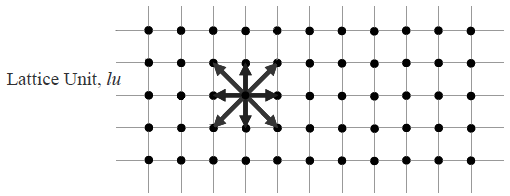
\includegraphics[scale=0.7]{d2q9.png}
	\caption{D2Q9 lattice and velocities. Adapted from \citep{sukop2006lattice}.}
	\label{fig:d2q9}
\end{figure}

Because particle mass is uniform (1 mass unit or mu in the simplest approach), these microscopic velocities and momenta are always effectively equivalent. The lattice unit (lu) is the fundamental measure of length in the LBM models and time steps (ts) are the time unit. 

The velocity magnitude of $e_1$ through $e_4$ is 1 lattice unit per time step or 1 lu ${ts}^{-1}$, and the velocity magnitude of $e_5$ through $e_8$ is $\sqrt{2}$ lu ${ts}^{-1}$. (While this is probably the most common velocity indexing scheme, be aware that others are in use.) These velocities are exceptionally convenient in that all of their $x$ and $y$ components are either 0 or \pm 1.
